\begin{enumerate}[label=\thesubsection.\arabic*, ref=\thesubsection.\theenumi]
\item
If tangents $PA$ and $PB$ drawn from an external point $P$ to a circle with centre $O$ are inclined to each other at an angle of $80^\circ$, then $\angle POA$ is equal to
\hfill (CBSE 2025 Set 2, Q.1)
\begin{enumerate}
	\begin{multicols}{4}
    \item $40^\circ$
    \item $50^\circ$
    \item $60^\circ$
    \item $80^\circ$
	\end{multicols}
\end{enumerate}
\solution
Take the centre $\vec{O} = \myvec{0 \\ 0}$ as the origin and $\vec{P} = \myvec{d \\ 0}$ on the $x$-axis. Let $r$ be the radius and $\phi = \angle POA$. The points of contact are symmetric about $OP$, so
\begin{align}
	\vec{A} = r\myvec{\cos\phi \\ \sin\phi}, \quad \vec{B} = r\myvec{\cos\phi \\ -\sin\phi}
\end{align}
The radius is perpendicular to the tangent at the point of contact,
\begin{align}
	\brak{\vec{A}-\vec{O}}^{\top}\brak{\vec{A}-\vec{P}} = 0 \implies \norm{\vec{A}}^2 = \vec{A}^{\top}\vec{P}
	\implies r^2 = rd\cos\phi \implies r = d\cos\phi
\end{align}
Hence the direction vectors of the tangents $PA$ and $PB$ are
\begin{align}
	\vec{A}-\vec{P} &= d\myvec{\cos^2\phi - 1 \\ \sin\phi\cos\phi} = d\sin\phi\myvec{-\sin\phi \\ \cos\phi}
	\\
	\vec{B}-\vec{P} &= d\myvec{\cos^2\phi - 1 \\ -\sin\phi\cos\phi} = d\sin\phi\myvec{-\sin\phi \\ -\cos\phi}
\end{align}
The unit direction vectors are $\vec{m}_1 = \myvec{-\sin\phi \\ \cos\phi}$ and $\vec{m}_2 = \myvec{-\sin\phi \\ -\cos\phi}$, so the angle between the tangents satisfies
\begin{align}
	\cos\angle APB = \vec{m}_1^{\top}\vec{m}_2 = \sin^2\phi - \cos^2\phi = -\cos 2\phi
\end{align}
Given $\angle APB = 80^\circ$,
\begin{align}
	\cos 2\phi = -\cos 80^\circ = \cos 100^\circ \implies \phi = 50^\circ
	\implies \angle POA = 50^\circ \quad \brak{\text{Option B}}
\end{align}
Taking $r = 2$, we get $d = \frac{r}{\cos 50^\circ} \approx 3.11$ and the points
\begin{align}
	\vec{O} = \myvec{0 \\ 0}, \quad \vec{P} = \myvec{3.11 \\ 0}, \quad
	\vec{A} = \myvec{1.29 \\ 1.53}, \quad \vec{B} = \myvec{1.29 \\ -1.53}
\end{align}
The following code verifies the solution
\begin{lstlisting}[frame=single, basicstyle=\rmfamily, escapeinside={(*@}{@*)}]
(*@\makebox[\dimexpr\linewidth-2\fboxsep-2\fboxrule\relax][c]{codes/1.c}@*)
\end{lstlisting}
The following code generates \figref{fig:CBSE25S2-q1}.
\begin{lstlisting}[frame=single, basicstyle=\rmfamily, escapeinside={(*@}{@*)}]
(*@\makebox[\dimexpr\linewidth-2\fboxsep-2\fboxrule\relax][c]{codes/1plot.py}@*)
\end{lstlisting}
\begin{figure}[H]
	\centering
	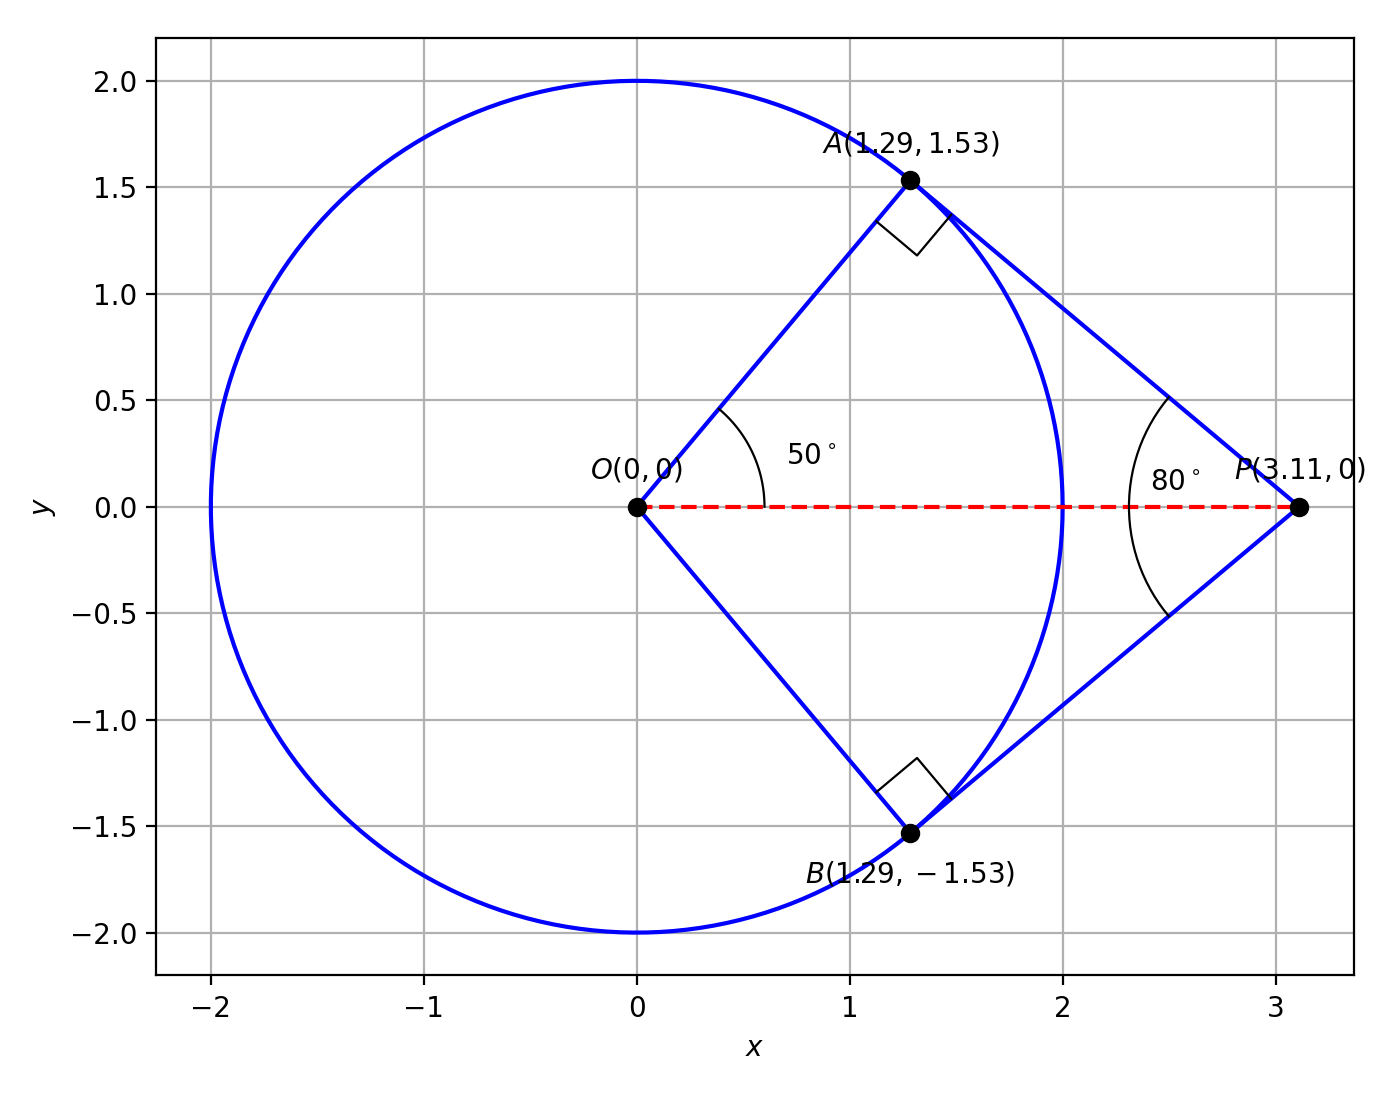
\includegraphics[width=0.6\linewidth]{figs/q1.png}
	\caption{Tangents $PA$ and $PB$ plotted from the coordinates of $\vec{O}$, $\vec{P}$, $\vec{A}$, $\vec{B}$}
	\label{fig:CBSE25S2-q1}
\end{figure}

\item
Two vertices of $\triangle PQR$ are $P\brak{-1,5}$ and $Q\brak{5,2}$. The coordinates of the point $R$ on $PQ$ which divides $PQ$ in the ratio $2:1$ are
\hfill (CBSE 2025 Set 2, Q.4)
\begin{enumerate}
	\begin{multicols}{4}
    \item $\brak{3,-3}$
    \item $\brak{5,5}$
    \item $\brak{3,3}$
    \item $\brak{5,1}$
	\end{multicols}
\end{enumerate}

\solution
Let $\vec{P} = \myvec{-1 \\ 5}$ and $\vec{Q} = \myvec{5 \\ 2}$. The displacement from $P$ to $Q$ is
\begin{align}
	\vec{Q} - \vec{P} = \myvec{6 \\ -3}
\end{align}
Since $PR : RQ = 2:1$, the point $R$ lies two-thirds of the way from $P$ to $Q$:
\begin{align}
	\vec{R} = \vec{P} + \frac{2}{3}\brak{\vec{Q}-\vec{P}} = \myvec{-1 \\ 5} + \myvec{4 \\ -2} = \myvec{3 \\ 3} \quad \brak{\text{Option C}}
\end{align}
The following code verifies the solution
\begin{lstlisting}[frame=single, basicstyle=\rmfamily, escapeinside={(*@}{@*)}]
(*@\makebox[\dimexpr\linewidth-2\fboxsep-2\fboxrule\relax][c]{codes/4.c}@*)
\end{lstlisting}
The following code generates \figref{fig:CBSE25S2-q4}.
\begin{lstlisting}[frame=single, basicstyle=\rmfamily, escapeinside={(*@}{@*)}]
(*@\makebox[\dimexpr\linewidth-2\fboxsep-2\fboxrule\relax][c]{codes/4plot.py}@*)
\end{lstlisting}
\begin{figure}[H]
	\centering
	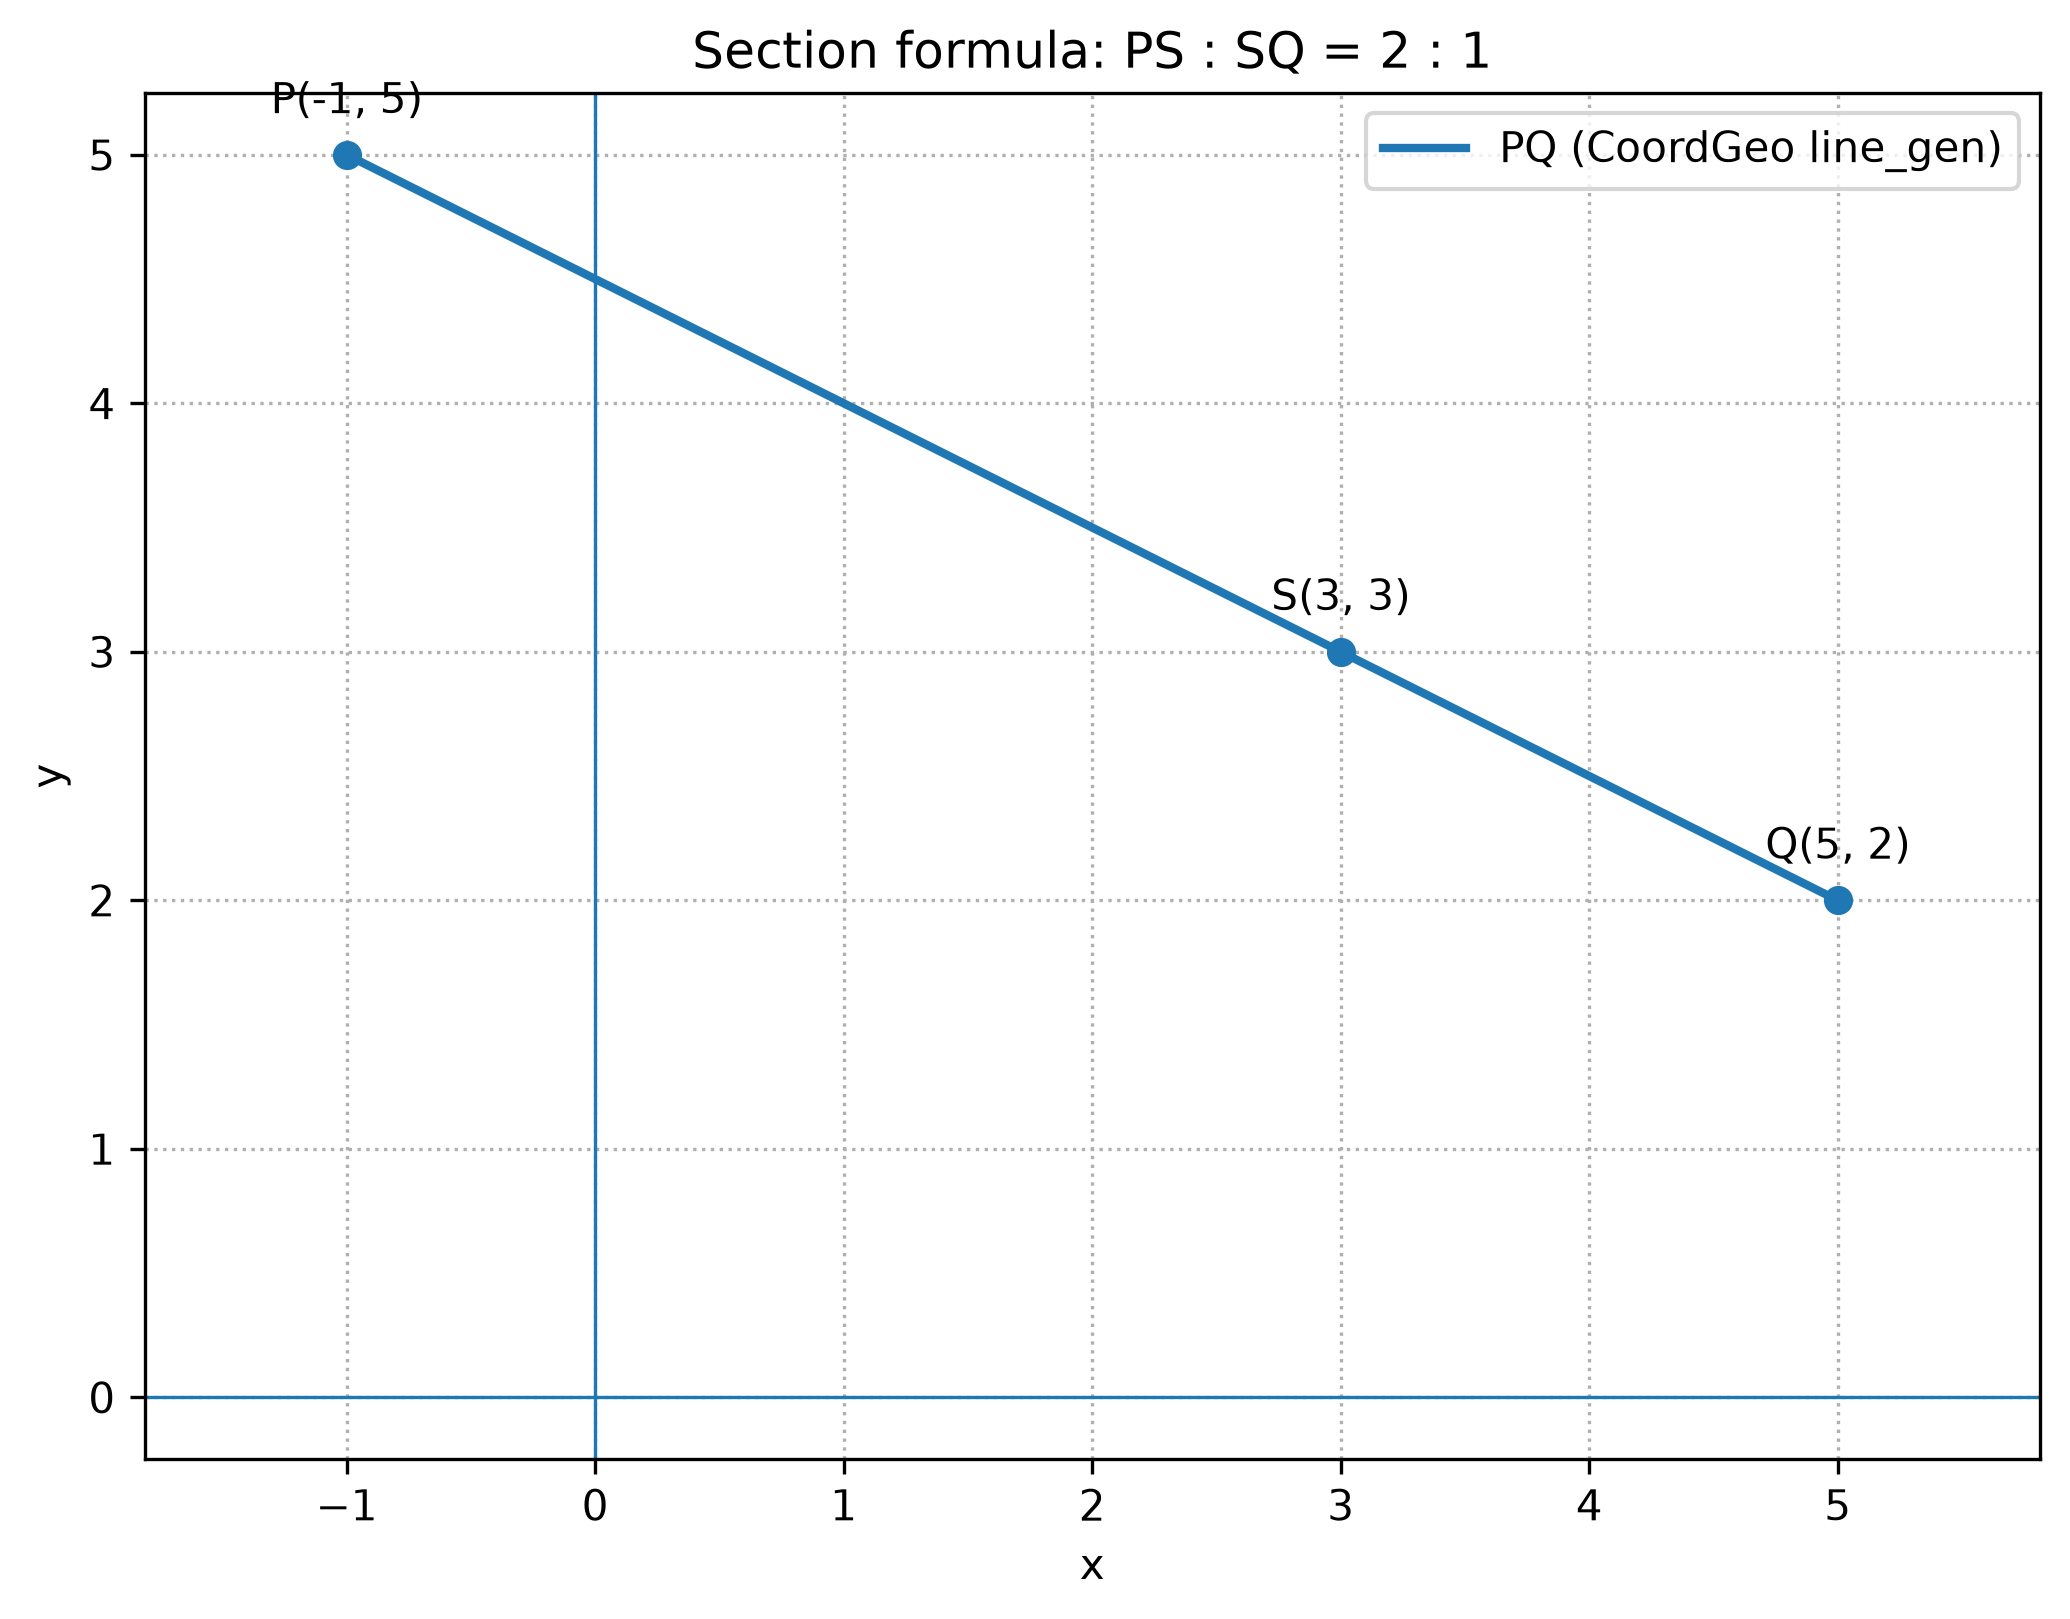
\includegraphics[width=0.5\linewidth]{figs/q4.png}
	\caption{Point $R$ dividing $PQ$ in the ratio $2:1$}
	\label{fig:CBSE25S2-q4}
\end{figure}

\item
If $\sin 4\theta = \frac{\sqrt{3}}{2}$, then $\frac{\theta}{3}$ is equal to
\hfill (CBSE 2025 Set 2, Q.5)
\begin{enumerate}
	\begin{multicols}{4}
    \item $60^\circ$
    \item $20^\circ$
    \item $15^\circ$
    \item $5^\circ$
	\end{multicols}
\end{enumerate}

\solution
Taking the principal (acute) value,
\begin{align}
	4\theta = \sin^{-1}\brak{\frac{\sqrt{3}}{2}} = 60^\circ
	\implies \theta = 15^\circ
	\implies \frac{\theta}{3} = 5^\circ \quad \brak{\text{Option D}}
\end{align}
The following code verifies the solution
\begin{lstlisting}[frame=single, basicstyle=\rmfamily, escapeinside={(*@}{@*)}]
(*@\makebox[\dimexpr\linewidth-2\fboxsep-2\fboxrule\relax][c]{codes/5.c}@*)
\end{lstlisting}

\item
The zeroes of the polynomial $p\brak{y} = 7y^2 - \frac{11}{3}y - \frac{2}{3}$ are
\hfill (CBSE 2025 Set 2, Q.6)
\begin{enumerate}
    \begin{multicols}{4}
        \item $\displaystyle -\frac{2}{3},-\frac{1}{7}$
        \item $\displaystyle -\frac{2}{7},-\frac{1}{3}$
        \item $\displaystyle \frac{2}{3},\frac{1}{7}$
        \item $\displaystyle \frac{2}{3},-\frac{1}{7}$
    \end{multicols}
\end{enumerate}

\solution
Multiplying by $3$, the zeroes of $p$ are the zeroes of
\begin{align}
	g\brak{y} = 21y^2 - 11y - 2, \quad g^{\prime}\brak{y} = 42y - 11
\end{align}
The Newton--Raphson iteration is
\begin{align}
	y_{n+1} = y_n - \frac{g\brak{y_n}}{g^{\prime}\brak{y_n}} = y_n - \frac{21y_n^2 - 11y_n - 2}{42y_n - 11}
\end{align}
Starting from $y_0 = 0.7$ and $y_0 = -0.2$, the iterations converge to
\begin{align}
	y = \frac{2}{3}, \quad y = -\frac{1}{7} \quad \brak{\text{Option D}}
\end{align}
which agree with the factorisation $g\brak{y} = \brak{3y-2}\brak{7y+1}$. The following code verifies the solution
\begin{lstlisting}[frame=single, basicstyle=\rmfamily, escapeinside={(*@}{@*)}]
(*@\makebox[\dimexpr\linewidth-2\fboxsep-2\fboxrule\relax][c]{codes/6.c}@*)
\end{lstlisting}
The following code generates \figref{fig:CBSE25S2-q6}.
\begin{lstlisting}[frame=single, basicstyle=\rmfamily, escapeinside={(*@}{@*)}]
(*@\makebox[\dimexpr\linewidth-2\fboxsep-2\fboxrule\relax][c]{codes/6plot.py}@*)
\end{lstlisting}
\begin{figure}[H]
	\centering
	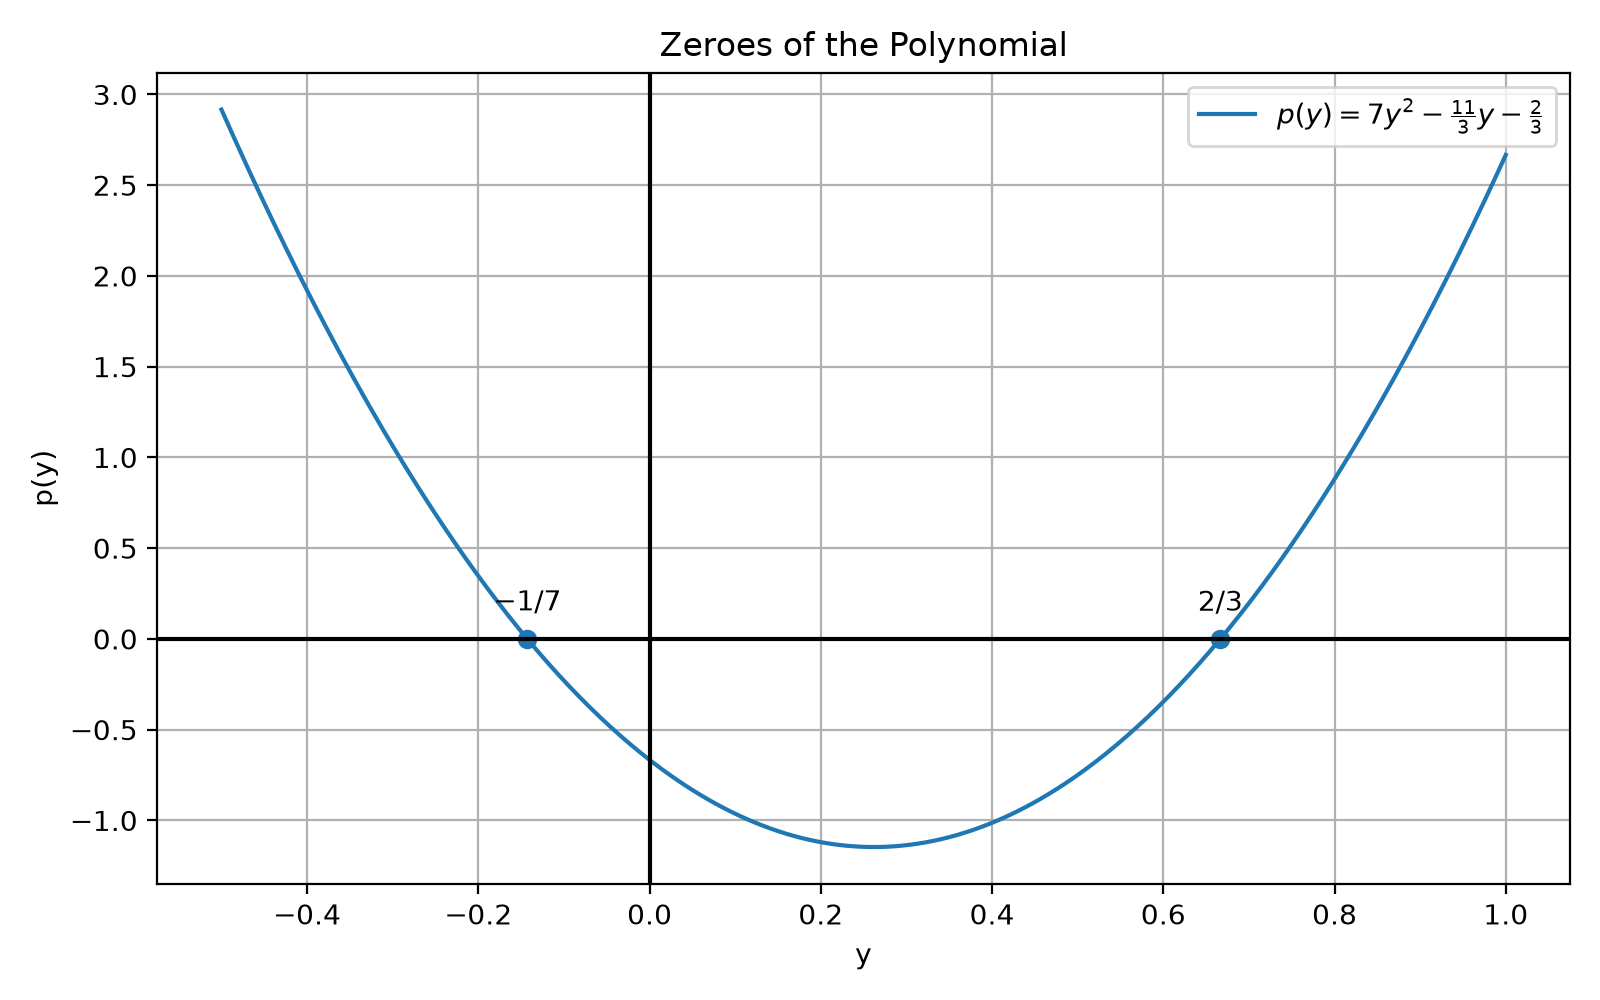
\includegraphics[width=0.6\linewidth]{figs/q6.png}
	\caption{Graph of $p\brak{y}$ and its zeroes}
	\label{fig:CBSE25S2-q6}
\end{figure}

\item
$AOBC$ is a rectangle whose three vertices are $A\brak{0,2}$, $O\brak{0,0}$ and $B\brak{4,0}$. The square of the length of its diagonal is
\hfill (CBSE 2025 Set 2, Q.8)
\begin{enumerate}
	\begin{multicols}{4}
    \item $36$
    \item $20$
    \item $16$
    \item $4$
	\end{multicols}
\end{enumerate}

\solution
The fourth vertex is $C\brak{4,2}$ and the diagonal is $AB$. With $\vec{A} = \myvec{0\\2}$, $\vec{B} = \myvec{4\\0}$,
\begin{align}
	\vec{B} - \vec{A} = \myvec{4 \\ -2}, \qquad
	\norm{\vec{B}-\vec{A}}^2 = \brak{\vec{B}-\vec{A}}^{\top}\brak{\vec{B}-\vec{A}} = 16 + 4 = 20 \quad \brak{\text{Option B}}
\end{align}
The following code verifies the solution
\begin{lstlisting}[frame=single, basicstyle=\rmfamily, escapeinside={(*@}{@*)}]
(*@\makebox[\dimexpr\linewidth-2\fboxsep-2\fboxrule\relax][c]{codes/8.c}@*)
\end{lstlisting}
The following code generates \figref{fig:CBSE25S2-q8}.
\begin{lstlisting}[frame=single, basicstyle=\rmfamily, escapeinside={(*@}{@*)}]
(*@\makebox[\dimexpr\linewidth-2\fboxsep-2\fboxrule\relax][c]{codes/8plot.py}@*)
\end{lstlisting}
\begin{figure}[H]
	\centering
	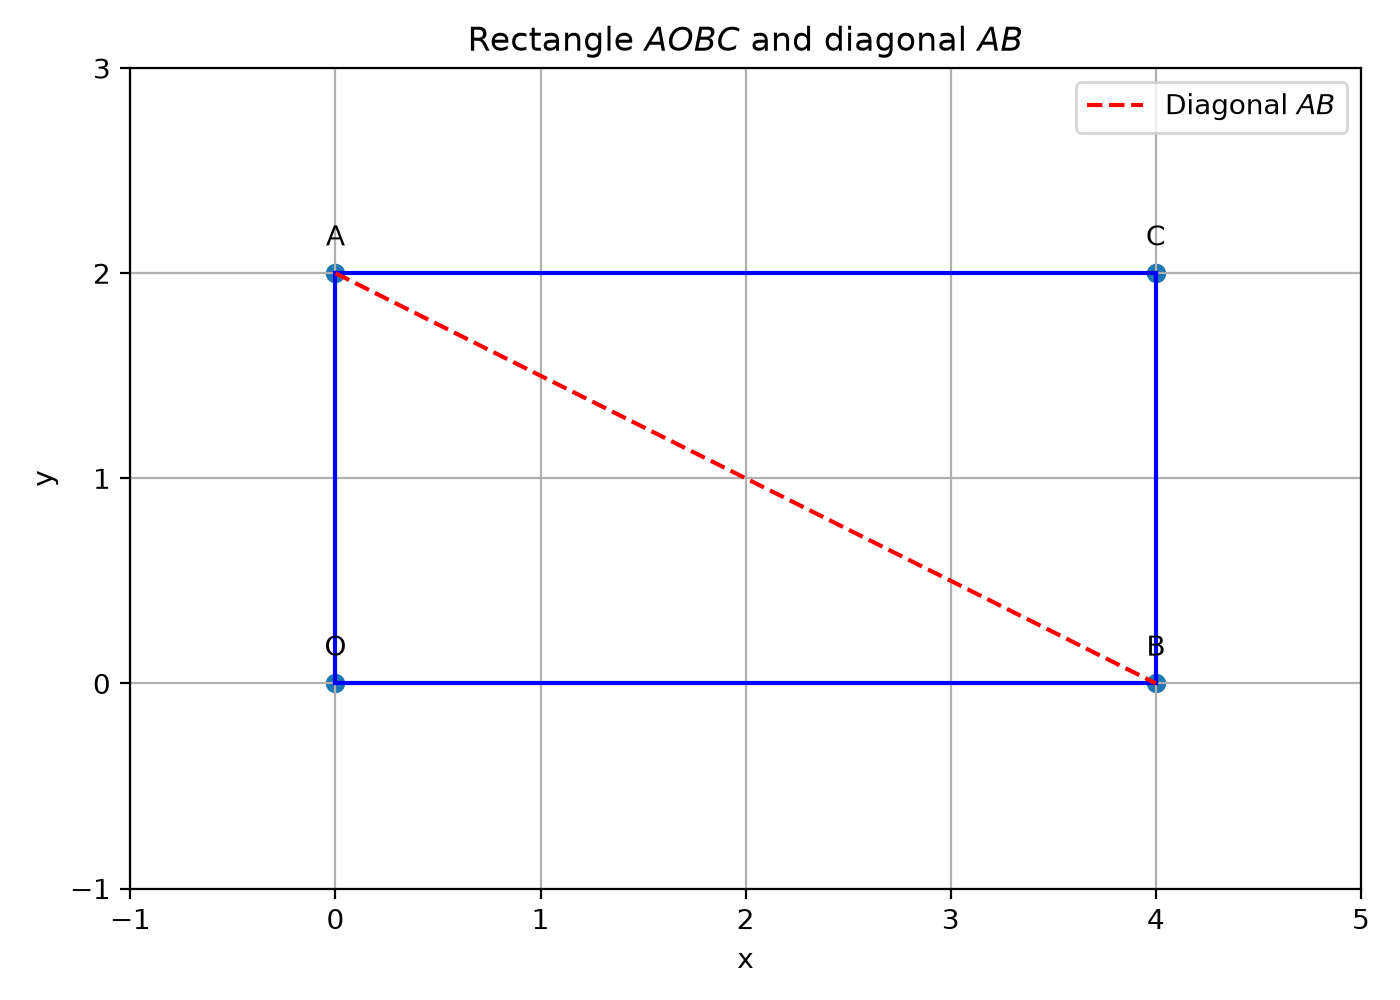
\includegraphics[width=0.55\linewidth]{figs/q8.png}
	\caption{Rectangle $AOBC$ and its diagonals}
	\label{fig:CBSE25S2-q8}
\end{figure}

\item
A die is thrown once. The probability of getting a number which is not a factor of $36$ is
\hfill (CBSE 2025 Set 2, Q.10)
\begin{enumerate}
	\begin{multicols}{4}
    \item $\frac{1}{2}$
    \item $\frac{2}{3}$
    \item $\frac{1}{6}$
    \item $\frac{5}{6}$
	\end{multicols}
\end{enumerate}

\solution
Let the outcome of the throw be $n$. The probability mass function of a fair die is
\begin{align}
	p\sbrak{n} &= \frac{1}{6}\brak{u\sbrak{n-1} - u\sbrak{n-7}}
	\\
	\implies P\brak{z} &= \sum_{n} p\sbrak{n}z^{-n} = \frac{1}{6}\brak{z^{-1} + z^{-2} + \cdots + z^{-6}}
\end{align}
where $u\sbrak{n}$ is the unit step. Define the indicator of the event $E$ (``not a factor of $36$''). Among $1,\dots,6$ only $5$ is not a factor of $36$, so
\begin{align}
	m\sbrak{n} = \delta\sbrak{n-5}, \quad M\brak{z} = z^{-5}
\end{align}
and $\pr{E} = \sum_n p\sbrak{n}m\sbrak{n}$. With the reversed sequence $h\sbrak{n} = m\sbrak{-n} = \delta\sbrak{n+5}$, whose transform is $H\brak{z} = z^{5}$, the convolution at $n=0$ gives exactly this sum:
\begin{align}
	\brak{p * h}\sbrak{0} = \sum_{k} p\sbrak{k}\,h\sbrak{-k} = \sum_{k} p\sbrak{k}\,m\sbrak{k} = \pr{E}
\end{align}
Convolution becomes multiplication in the $z$-domain,
\begin{align}
	Y\brak{z} = P\brak{z}H\brak{z} = \frac{1}{6}\sum_{n=1}^{6} z^{5-n}
	= \frac{1}{6}\brak{z^{4} + z^{3} + z^{2} + z + 1 + z^{-1}}
\end{align}
and $\brak{p*h}\sbrak{0}$ is the coefficient of $z^{0}$. Therefore,
\begin{align}
	\pr{E} = \frac{1}{6} \quad \brak{\text{Option C}}
\end{align}
The following code verifies the solution
\begin{lstlisting}[frame=single, basicstyle=\rmfamily, escapeinside={(*@}{@*)}]
(*@\makebox[\dimexpr\linewidth-2\fboxsep-2\fboxrule\relax][c]{codes/10.c}@*)
\end{lstlisting}

\item
In the figure, $\angle BAC = 90^\circ$ and $AD \perp BC$. If $BC = 16$ cm and $DC = 4$ cm, then $AC = x$ is equal to
\hfill (CBSE 2025 Set 2, Q.11)
\begin{enumerate}
    \begin{multicols}{4}
        \item $4\text{ cm}$
        \item $5\text{ cm}$
        \item $8\text{ cm}$
        \item $3\text{ cm}$
    \end{multicols}
\end{enumerate}
\solution
Take $\vec{B} = \myvec{0\\0}$, $\vec{C} = \myvec{16\\0}$. Then $BD = 16-4 = 12$, so $\vec{D} = \myvec{12\\0}$ and, since $AD \perp BC$, $\vec{A} = \myvec{12\\h}$. As $\angle BAC = 90^\circ$,
\begin{align}
	\brak{\vec{B}-\vec{A}}^{\top}\brak{\vec{C}-\vec{A}} &= 0
	\\
	\myvec{-12 & -h}\myvec{4 \\ -h} = -48 + h^2 &= 0 \implies h^2 = 48
\end{align}
Hence,
\begin{align}
	x^2 = \norm{\vec{C}-\vec{A}}^2 = 4^2 + h^2 = 64 \implies x = 8 \text{ cm} \quad \brak{\text{Option C}}
\end{align}
The following code verifies the solution
\begin{lstlisting}[frame=single, basicstyle=\rmfamily, escapeinside={(*@}{@*)}]
(*@\makebox[\dimexpr\linewidth-2\fboxsep-2\fboxrule\relax][c]{codes/11.c}@*)
\end{lstlisting}
The following code generates \figref{fig:CBSE25S2-q11}.
\begin{lstlisting}[frame=single, basicstyle=\rmfamily, escapeinside={(*@}{@*)}]
(*@\makebox[\dimexpr\linewidth-2\fboxsep-2\fboxrule\relax][c]{codes/11plot.py}@*)
\end{lstlisting}
\begin{figure}[H]
	\centering
	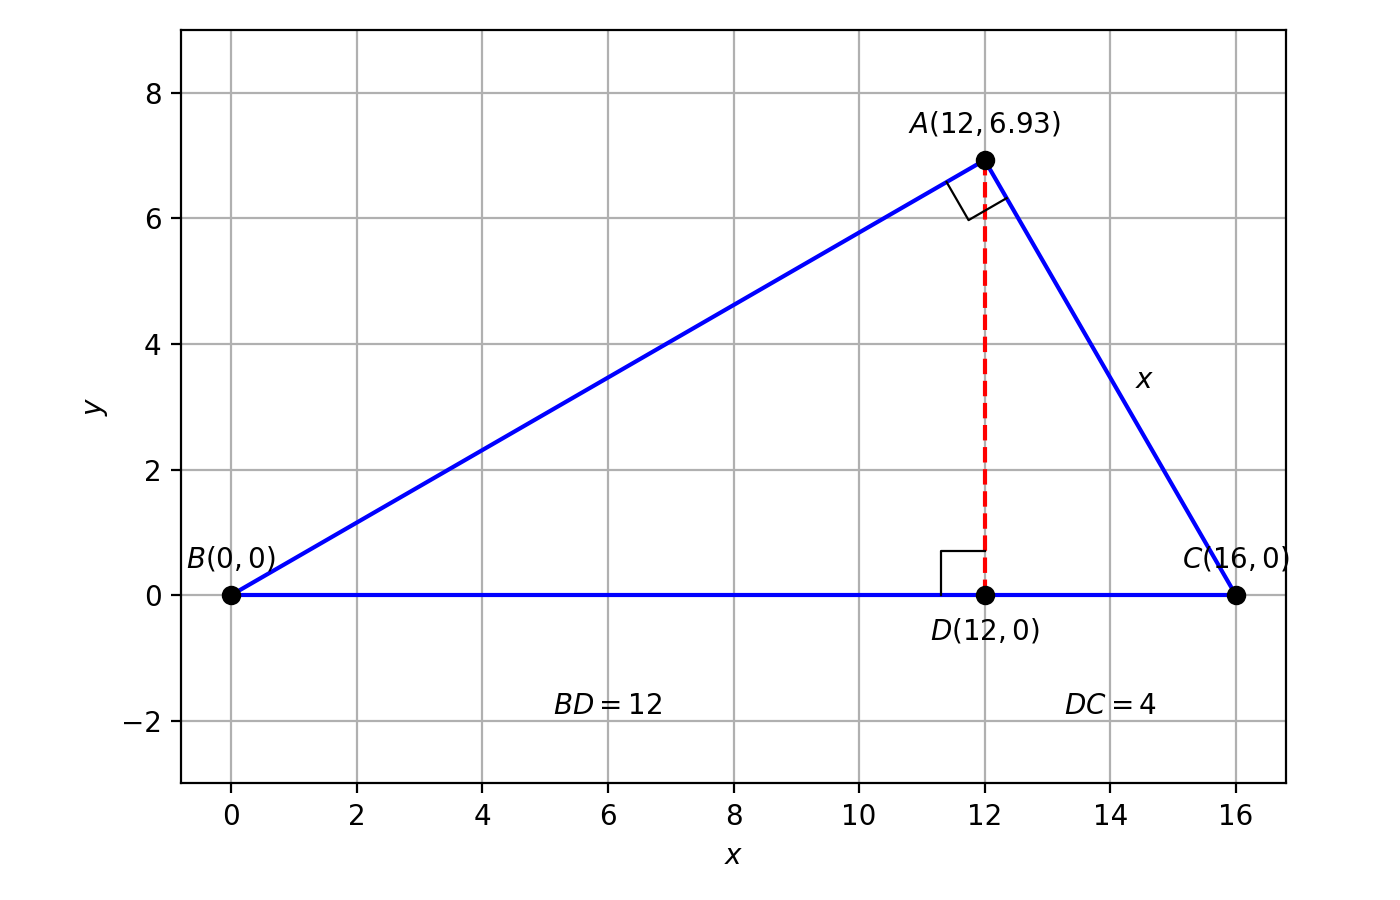
\includegraphics[width=0.6\linewidth]{figs/q11.png}
	\caption{Right triangle $ABC$ with altitude $AD$, plotted from the coordinates of $\vec{B}$, $\vec{C}$, $\vec{D}$, $\vec{A}$}
	\label{fig:CBSE25S2-q11}
\end{figure}

\item
The mid-point of the line segment joining $\brak{a,4}$ and $\brak{2,2b}$ is $\brak{2,6}$. Then $a + b$ is equal to
\hfill (CBSE 2025 Set 2, Q.15)
\begin{enumerate}
    \begin{multicols}{4}
        \item $6$
        \item $7$
        \item $8$
        \item $16$
    \end{multicols}
\end{enumerate}

\solution
The mid-point is the average of the position vectors:
\begin{align}
	\myvec{2 \\ 6} = \frac{1}{2}\brak{\myvec{a \\ 4} + \myvec{2 \\ 2b}}
	\implies \frac{a+2}{2} = 2, \quad \frac{4+2b}{2} = 6
	\implies a = 2, \quad b = 4
\end{align}
Therefore $a + b = 6$ (Option A). The following code verifies the solution
\begin{lstlisting}[frame=single, basicstyle=\rmfamily, escapeinside={(*@}{@*)}]
(*@\makebox[\dimexpr\linewidth-2\fboxsep-2\fboxrule\relax][c]{codes/15.c}@*)
\end{lstlisting}
The following code generates \figref{fig:CBSE25S2-q15}.
\begin{lstlisting}[frame=single, basicstyle=\rmfamily, escapeinside={(*@}{@*)}]
(*@\makebox[\dimexpr\linewidth-2\fboxsep-2\fboxrule\relax][c]{codes/15plot.py}@*)
\end{lstlisting}
\begin{figure}[H]
	\centering
	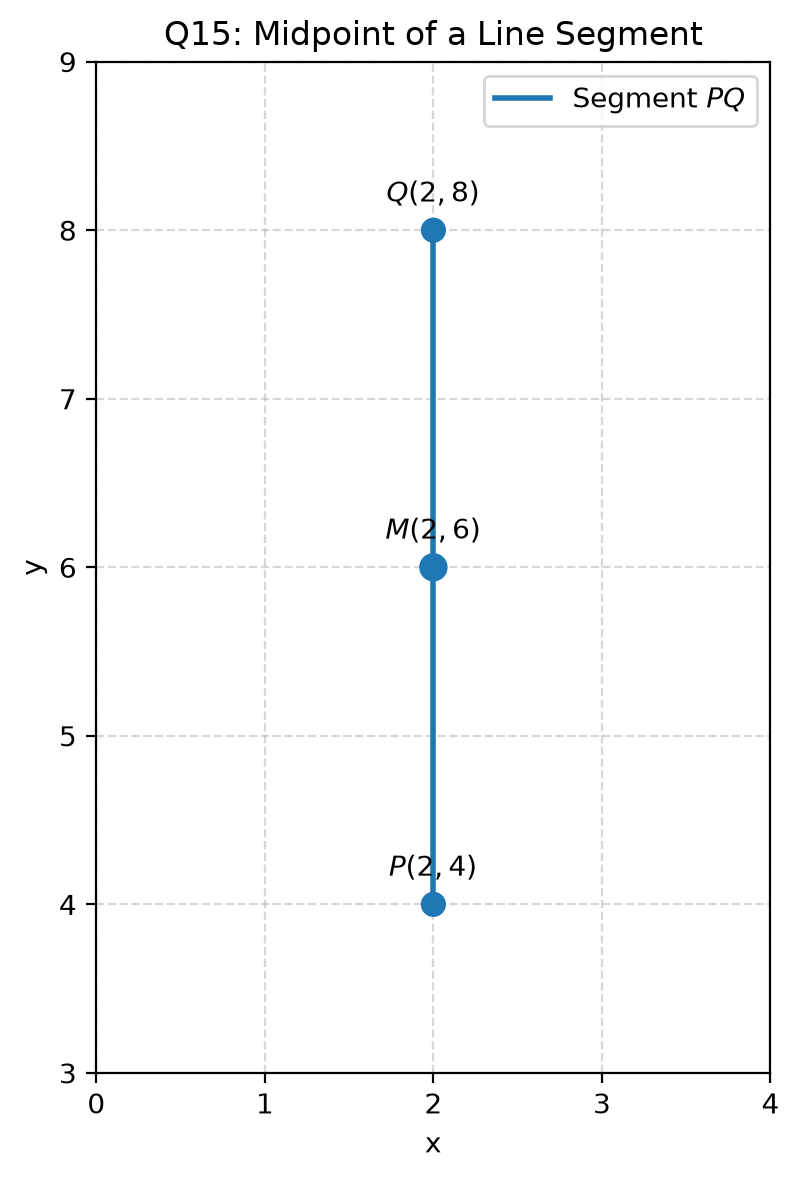
\includegraphics[width=0.45\linewidth]{figs/q15.png}
	\caption{Segment $PQ$ and its mid-point $M$}
	\label{fig:CBSE25S2-q15}
\end{figure}

\item
 $\angle M = \angle B = 130^\circ$ and $\angle N = 28^\circ$. If $LM = 45$ cm, $MN = 63$ cm, $LN = 72$ cm and $AB = 5$ cm, then $AC$ is equal to
\hfill (CBSE 2025 Set 2, Q.17)
\begin{enumerate}
    \begin{multicols}{4}
        \item $16\text{ cm}$
        \item $7\text{ cm}$
        \item $8\text{ cm}$
        \item $4\text{ cm}$
    \end{multicols}
\end{enumerate}
\solution
In $\triangle LMN$, $\angle L = 180^\circ - 130^\circ - 28^\circ = 22^\circ = \angle A$. Since $\angle A = \angle L$ and $\angle B = \angle M$, by AA similarity
\begin{align}
	\triangle LMN \sim \triangle ABC \quad \brak{L \leftrightarrow A,\ M \leftrightarrow B,\ N \leftrightarrow C}
\end{align}
The scale factor is $k = \frac{AB}{LM} = \frac{5}{45} = \frac{1}{9}$, so
\begin{align}
	AC = k \cdot LN = \frac{72}{9} = 8 \text{ cm} \quad \brak{\text{Option C}}
\end{align}
The following code verifies the solution
\begin{lstlisting}[frame=single, basicstyle=\rmfamily, escapeinside={(*@}{@*)}]
(*@\makebox[\dimexpr\linewidth-2\fboxsep-2\fboxrule\relax][c]{codes/17.c}@*)
\end{lstlisting}
The following code generates \figref{fig:CBSE25S2-q17}. The triangle $LMN$ is drawn from the given angles with $LN = 72$ cm, and $ABC$ is its image under the scale factor $\frac{1}{9}$; the figure is not to scale with respect to $MN$.
\begin{lstlisting}[frame=single, basicstyle=\rmfamily, escapeinside={(*@}{@*)}]
(*@\makebox[\dimexpr\linewidth-2\fboxsep-2\fboxrule\relax][c]{codes/17plot.py}@*)
\end{lstlisting}
\begin{figure}[H]
	\centering
	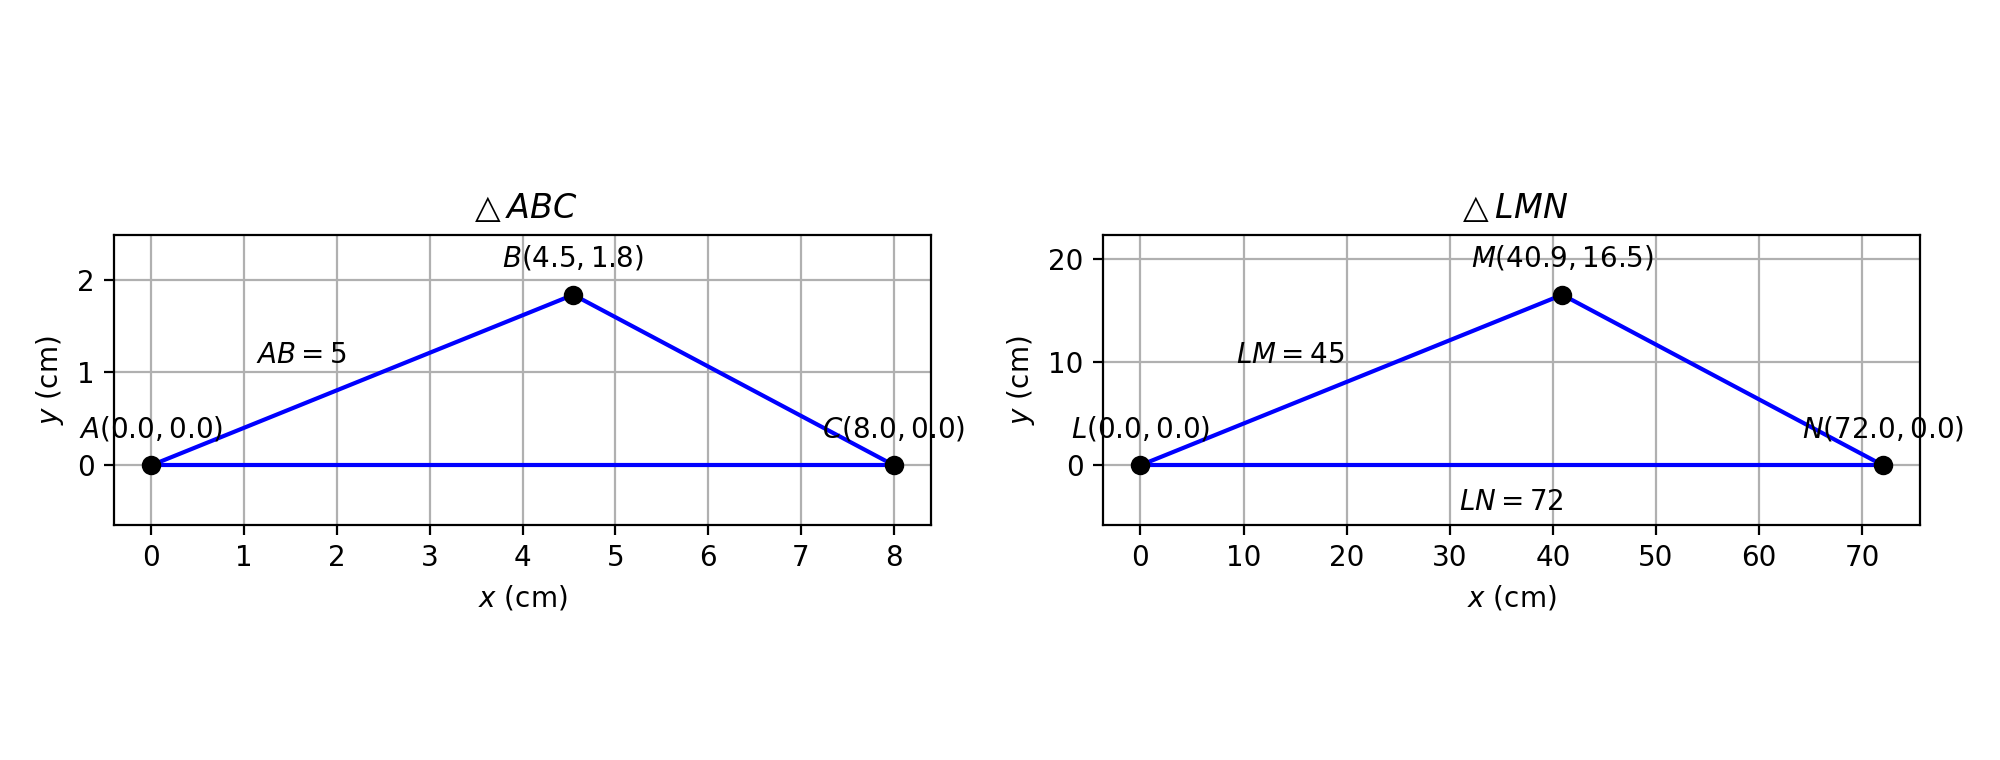
\includegraphics[width=\linewidth]{figs/q17.png}
	\caption{Triangles $ABC$ and $LMN$ plotted from coordinates}
	\label{fig:CBSE25S2-q17}
\end{figure}

\item
$\triangle DEF$ and $\triangle PQR$ are such that $\angle D = \angle Q$ and $\angle E = \angle R$. Which of the following proportions is \underline{not} true?
\hfill (CBSE 2025 Set 2, Q.18)
\begin{enumerate}
	\begin{multicols}{4}
    \item $\frac{DE}{QR} = \frac{DF}{PQ}$
    \item $\frac{EF}{RP} = \frac{DF}{PQ}$
    \item $\frac{EF}{RP} = \frac{DE}{QR}$
    \item $\frac{DE}{PQ} = \frac{EF}{RP}$
	\end{multicols}
\end{enumerate}

\solution
By AA similarity, $\triangle DEF \sim \triangle QRP$ with $D \leftrightarrow Q$, $E \leftrightarrow R$, $F \leftrightarrow P$. Corresponding sides are proportional:
\begin{align}
	\frac{DE}{QR} = \frac{EF}{RP} = \frac{DF}{QP}
\end{align}
Options A, B and C compare corresponding sides. Option D compares $DE$ with $PQ$, which are not corresponding sides. Hence the proportion that is not true is Option D. The following code checks all four options on a pair of similar triangles
\begin{lstlisting}[frame=single, basicstyle=\rmfamily, escapeinside={(*@}{@*)}]
(*@\makebox[\dimexpr\linewidth-2\fboxsep-2\fboxrule\relax][c]{codes/18.c}@*)
\end{lstlisting}

\item
If $\alpha$ and $\beta$ are the zeroes of the polynomial $x^2 - 2x - 1$, find the value of $\frac{1}{2\alpha} + \frac{1}{2\beta} + 3\alpha\beta$.
\hfill (CBSE 2025 Set 2, Q.21(b))

\solution
Let $f\brak{x} = x^2 - 2x - 1$, so $f^{\prime}\brak{x} = 2x - 2$. The Newton--Raphson iteration is
\begin{align}
	x_{n+1} = x_n - \frac{x_n^2 - 2x_n - 1}{2x_n - 2}
\end{align}
Starting from $x_0 = 2.5$ and $x_0 = -0.5$ gives
\begin{align}
	\alpha = 1 + \sqrt{2}, \quad \beta = 1 - \sqrt{2}
\end{align}
From the sum and product of zeroes, $\alpha + \beta = 2$ and $\alpha\beta = -1$, so
\begin{align}
	\frac{1}{2\alpha} + \frac{1}{2\beta} + 3\alpha\beta = \frac{\alpha+\beta}{2\alpha\beta} + 3\alpha\beta = \frac{2}{-2} - 3 = -4
\end{align}
The following code verifies the solution
\begin{lstlisting}[frame=single, basicstyle=\rmfamily, escapeinside={(*@}{@*)}]
(*@\makebox[\dimexpr\linewidth-2\fboxsep-2\fboxrule\relax][c]{codes/21.c}@*)
\end{lstlisting}
The following code generates \figref{fig:CBSE25S2-q21b}.
\begin{lstlisting}[frame=single, basicstyle=\rmfamily, escapeinside={(*@}{@*)}]
(*@\makebox[\dimexpr\linewidth-2\fboxsep-2\fboxrule\relax][c]{codes/21plot.py}@*)
\end{lstlisting}
\begin{figure}[H]
	\centering
	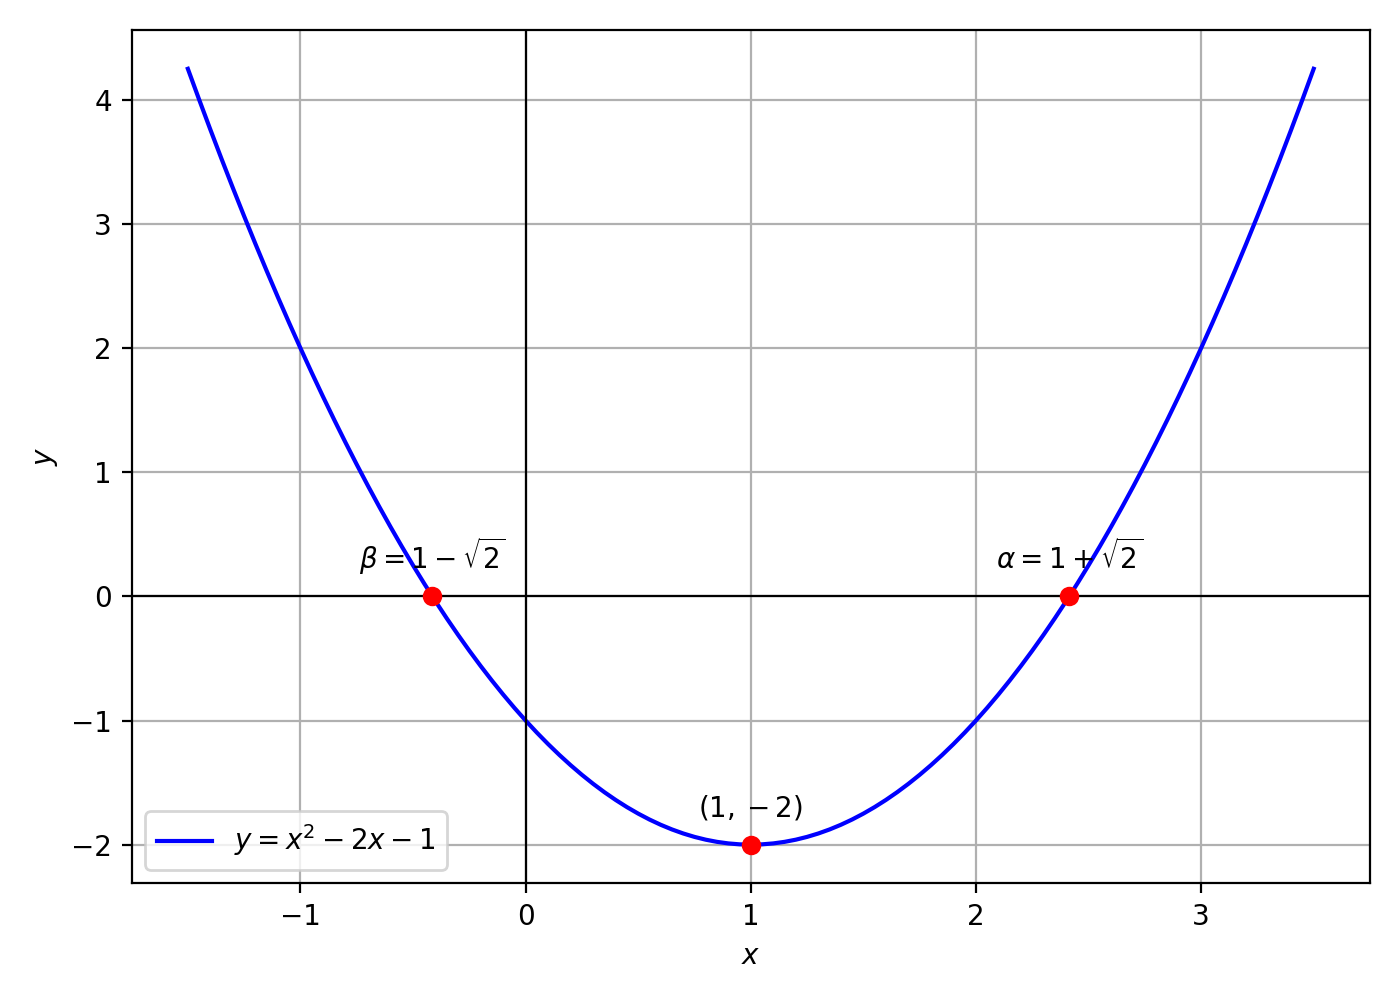
\includegraphics[width=0.6\linewidth]{figs/q21b.png}
	\caption{Graph of $y = x^2 - 2x - 1$ with zeroes $\alpha$ and $\beta$}
	\label{fig:CBSE25S2-q21b}
\end{figure}

\item
In a school, $65\%$ of the students have black eyes, $25\%$ have brown eyes and the rest have blue eyes. A student is chosen at random. Find the probability that the student has (a) blue eyes, (b) brown or black eyes.
\hfill (CBSE 2025 Set 2, Q.27)

\solution
Let $n = 0, 1, 2$ denote black, brown and blue eyes. The probability of blue eyes is $1 - 0.65 - 0.25 = 0.10$, so
\begin{align}
	p\sbrak{n} &= 0.65\,\delta\sbrak{n} + 0.25\,\delta\sbrak{n-1} + 0.10\,\delta\sbrak{n-2}
	\\
	\implies P\brak{z} &= 0.65 + 0.25z^{-1} + 0.10z^{-2}
\end{align}
For an event with indicator $m\sbrak{n}$, let $h\sbrak{n} = m\sbrak{-n}$. As in the previous problem,
\begin{align}
	\pr{E} = \sum_{k} p\sbrak{k}\,m\sbrak{k} = \brak{p * h}\sbrak{0}
\end{align}
which is the coefficient of $z^{0}$ in $P\brak{z}H\brak{z}$.

\textbf{(a) Blue eyes:} $m\sbrak{n} = \delta\sbrak{n-2}$, so $h\sbrak{n} = \delta\sbrak{n+2}$ and $H\brak{z} = z^{2}$,
\begin{align}
	P\brak{z}H\brak{z} &= 0.65z^{2} + 0.25z + 0.10
	\\
	\implies \pr{\text{blue}} &= 0.10
\end{align}
\textbf{(b) Brown or black eyes:} $m\sbrak{n} = \delta\sbrak{n} + \delta\sbrak{n-1}$, so $h\sbrak{n} = \delta\sbrak{n} + \delta\sbrak{n+1}$ and $H\brak{z} = 1 + z$,
\begin{align}
	P\brak{z}H\brak{z} &= 0.65z + 0.90 + 0.35z^{-1} + 0.10z^{-2}
	\\
	\implies \pr{\text{brown or black}} &= 0.90
\end{align}
The following code verifies the solution
\begin{lstlisting}[frame=single, basicstyle=\rmfamily, escapeinside={(*@}{@*)}]
(*@\makebox[\dimexpr\linewidth-2\fboxsep-2\fboxrule\relax][c]{codes/27.c}@*)
\end{lstlisting}

\item
In the figure, $PC$ is a tangent to the circle at $C$ and $AB$ is a diameter which, when extended, meets the tangent at $P$. If $\angle PCA = 110^\circ$, find $\angle CBA$ and $\angle BCO$.
\hfill (CBSE 2025 Set 2, Q.29)

\solution
Since $AB$ is a diameter, $\angle ACB = 90^\circ$. As $P$ lies beyond $B$,
\begin{align}
	\angle PCA = \angle PCB + \angle BCA \implies \angle PCB = 110^\circ - 90^\circ = 20^\circ
\end{align}
By the tangent--chord theorem, $\angle CAB = \angle PCB = 20^\circ$. In $\triangle ABC$,
\begin{align}
	\angle CBA = 90^\circ - 20^\circ = 70^\circ
\end{align}
Since $OB = OC$, $\triangle OBC$ is isosceles and
\begin{align}
	\angle BCO = \angle CBO = 70^\circ
\end{align}
The following code verifies the solution
\begin{lstlisting}[frame=single, basicstyle=\rmfamily, escapeinside={(*@}{@*)}]
(*@\makebox[\dimexpr\linewidth-2\fboxsep-2\fboxrule\relax][c]{codes/29.c}@*)
\end{lstlisting}
The following code generates \figref{fig:CBSE25S2-q29}.
\begin{lstlisting}[frame=single, basicstyle=\rmfamily, escapeinside={(*@}{@*)}]
(*@\makebox[\dimexpr\linewidth-2\fboxsep-2\fboxrule\relax][c]{codes/29plot.py}@*)
\end{lstlisting}
\begin{figure}[H]
	\centering
	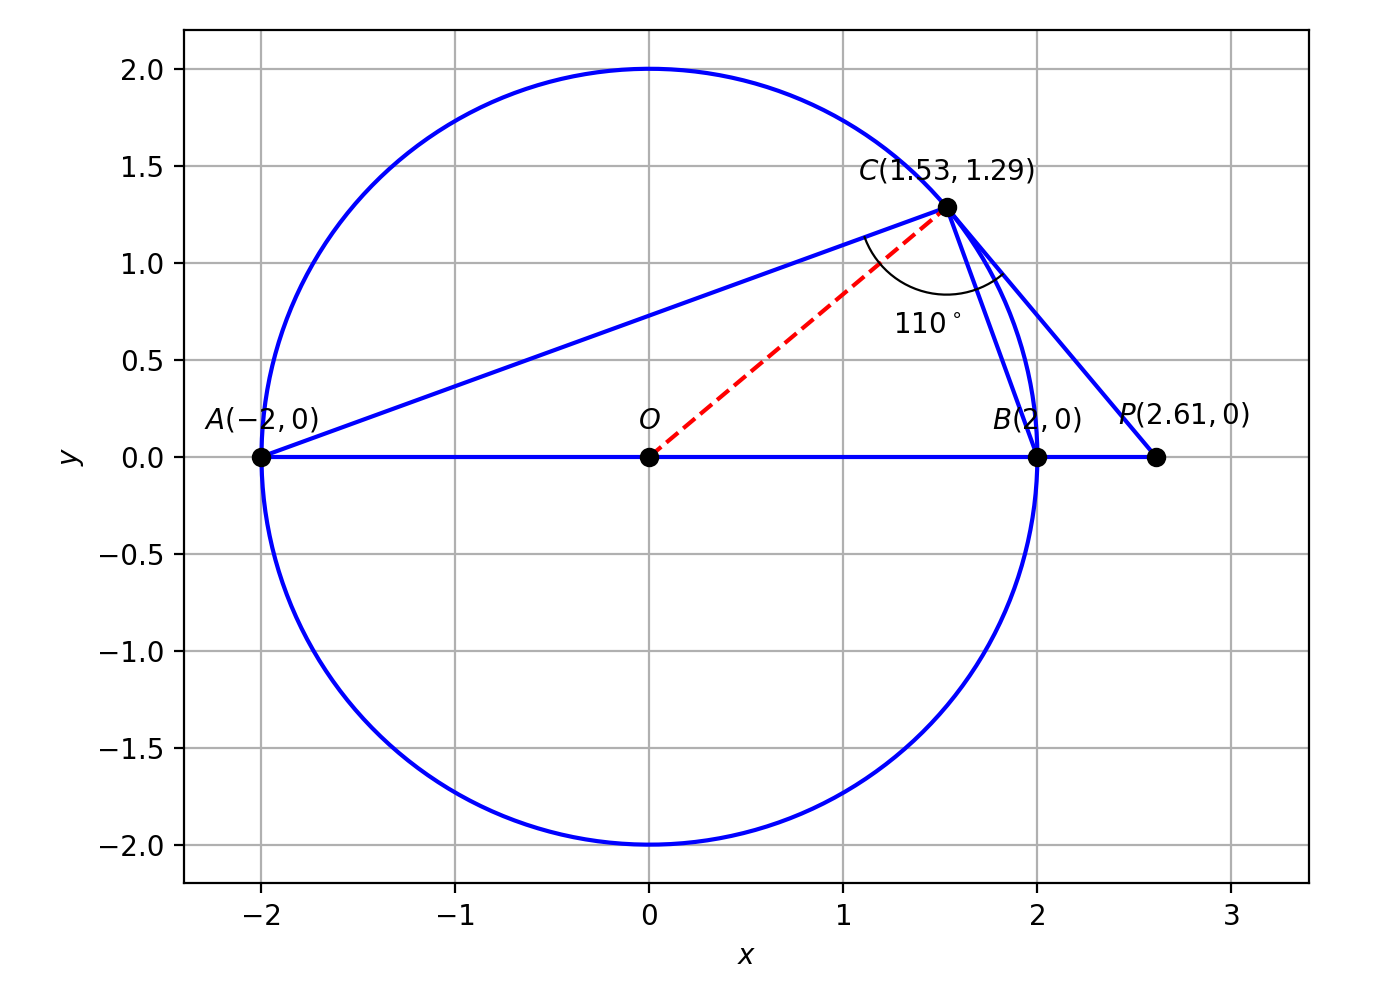
\includegraphics[width=0.6\linewidth]{figs/q29.png}
	\caption{Tangent $PC$ and diameter $AB$, plotted from the coordinates of $\vec{A}$, $\vec{B}$, $\vec{C}$, $\vec{P}$}
	\label{fig:CBSE25S2-q29}
\end{figure}

\item
Find the coordinates of the points which divide the line segment joining $A\brak{-2,2}$ and $B\brak{2,8}$ into four equal parts.
\hfill (CBSE 2025 Set 2, Q.31(b))

\solution
With $\vec{A} = \myvec{-2\\2}$ and $\vec{B} = \myvec{2\\8}$, $\vec{B}-\vec{A} = \myvec{4\\6}$. The division points are $\vec{A} + \frac{k}{4}\brak{\vec{B}-\vec{A}}$ for $k = 1,2,3$:
\begin{align}
	\vec{P} = \myvec{-1 \\ 3.5}, \quad \vec{Q} = \myvec{0 \\ 5}, \quad \vec{R} = \myvec{1 \\ 6.5}
\end{align}
The following code verifies the solution
\begin{lstlisting}[frame=single, basicstyle=\rmfamily, escapeinside={(*@}{@*)}]
(*@\makebox[\dimexpr\linewidth-2\fboxsep-2\fboxrule\relax][c]{codes/31.c}@*)
\end{lstlisting}
The following code generates \figref{fig:CBSE25S2-q31b}.
\begin{lstlisting}[frame=single, basicstyle=\rmfamily, escapeinside={(*@}{@*)}]
(*@\makebox[\dimexpr\linewidth-2\fboxsep-2\fboxrule\relax][c]{codes/31plot.py}@*)
\end{lstlisting}
\begin{figure}[H]
	\centering
	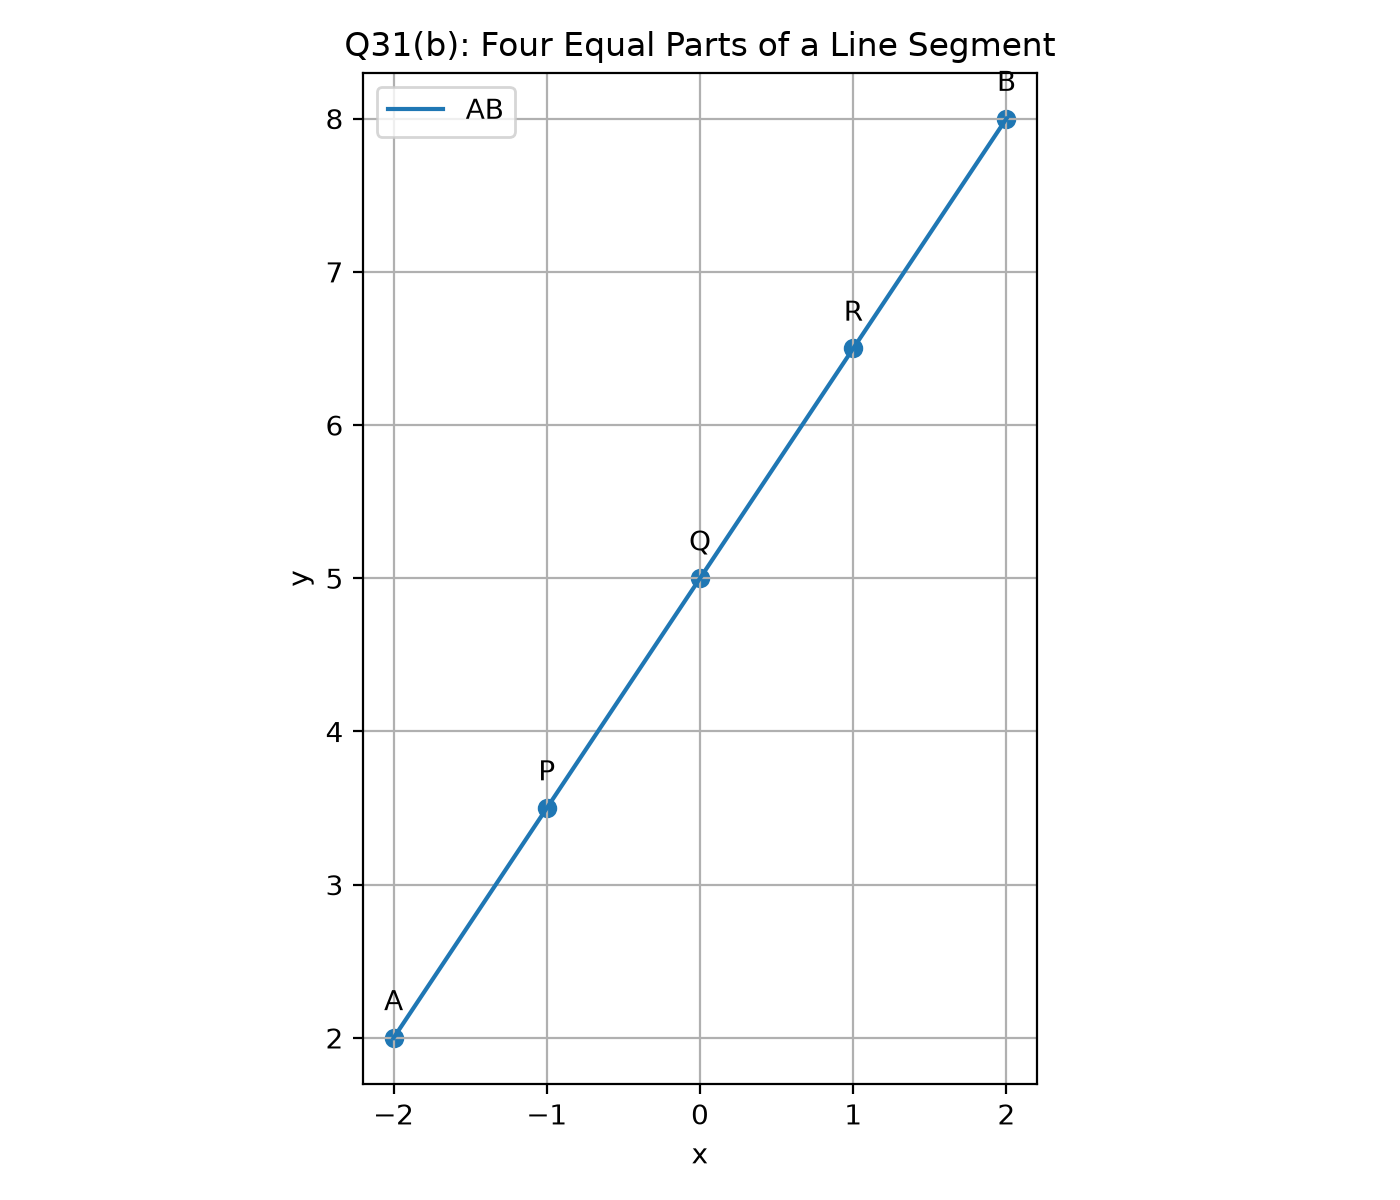
\includegraphics[width=0.5\linewidth]{figs/q31b.png}
	\caption{Division of $AB$ into four equal parts}
	\label{fig:CBSE25S2-q31b}
\end{figure}

\item
The $n^{\text{th}}$ term of an AP is $4$, its common difference is $2$ and the sum of its first $n$ terms is $-14$. Find $n$, the first term, and the sum of the first $20$ terms.
\hfill (CBSE 2025 Set 2, Q.32(a))

\solution
Let $u\sbrak{n}$ be the unit step function, $u\sbrak{n} = 1$ for $n \ge 0$ and $0$ otherwise. The AP with first term $a$ and common difference $d$ is the causal sequence
\begin{align}
	x\sbrak{n} = \brak{a + \brak{n-1}d}\,u\sbrak{n-1}
\end{align}
so that $x\sbrak{n} = a_n$ for $n \ge 1$ and $x\sbrak{n} = 0$ for $n \le 0$. Since $u\sbrak{n-k} = 1$ only for $k \le n$, the sum of the first $n$ terms is the convolution of $x$ with the unit step,
\begin{align}
	S\sbrak{n} = \sum_{k} x\sbrak{k}\,u\sbrak{n-k} = \brak{x * u}\sbrak{n}
	= \brak{na + \frac{n\brak{n-1}}{2}d}\,u\sbrak{n-1}
\end{align}
Here $d = 2$ and $x\sbrak{n} = 4$, so $a + 2\brak{n-1} = 4$ gives $a = 6 - 2n$. For $n \ge 1$,
\begin{align}
	S\sbrak{n} = n\brak{6 - 2n} + n\brak{n-1} &= n\brak{5 - n} = -14
	\\
	\implies n^2 - 5n - 14 &= 0 \implies \brak{n-7}\brak{n+2} = 0
\end{align}
The step $u\sbrak{n-1}$ requires $n \ge 1$, so $n = 7$ and $a = 6 - 14 = -8$. Then
\begin{align}
	S\sbrak{20} = 20\brak{-8} + \frac{20 \cdot 19}{2}\brak{2} = -160 + 380 = 220
\end{align}
The following code verifies the solution
\begin{lstlisting}[frame=single, basicstyle=\rmfamily, escapeinside={(*@}{@*)}]
(*@\makebox[\dimexpr\linewidth-2\fboxsep-2\fboxrule\relax][c]{codes/32a.c}@*)
\end{lstlisting}

\item
A man lent part of his money at $10\%$ per annum and the rest at $15\%$ per annum. His yearly interest was \rupee 1900. Had he interchanged the two rates, he would have earned \rupee 200 more. Find the two amounts.
\hfill (CBSE 2025 Set 2, Q.34)

\solution
Let $x$ and $y$ be the amounts lent at $10\%$ and $15\%$. Then
\begin{align}
	0.10x + 0.15y &= 1900 \\
	0.15x + 0.10y &= 2100
\end{align}
The augmented matrix of $\vec{A}\vec{x} = \vec{b}$ is $\myvec{\vec{A} & \vec{b}}$. Using Gaussian elimination (Gauss--Jordan row reduction),
\begin{align}
	\myvec{0.10 & 0.15 & 1900 \\ 0.15 & 0.10 & 2100}
	&\xleftrightarrow[]{R_1 \leftarrow 10R_1}
	\myvec{1 & 1.5 & 19000 \\ 0.15 & 0.10 & 2100}
	\\
	&\xleftrightarrow[]{R_2 \leftarrow R_2 - 0.15R_1}
	\myvec{1 & 1.5 & 19000 \\ 0 & -0.125 & -750}
	\\
	&\xleftrightarrow[]{R_2 \leftarrow R_2/\brak{-0.125}}
	\myvec{1 & 1.5 & 19000 \\ 0 & 1 & 6000}
	\\
	&\xleftrightarrow[]{R_1 \leftarrow R_1 - 1.5R_2}
	\myvec{1 & 0 & 10000 \\ 0 & 1 & 6000}
\end{align}
Both $\vec{A}$ and $\myvec{\vec{A} & \vec{b}}$ have two non-zero rows, so
\begin{align}
	\rank\brak{\vec{A}} = \rank\myvec{\vec{A} & \vec{b}} = 2 = \text{number of unknowns}
\end{align}
Hence the system is consistent with a unique solution,
\begin{align}
	\vec{x} = \myvec{x \\ y} = \myvec{10000 \\ 6000}
\end{align}
The amounts are \rupee 10000 at $10\%$ and \rupee 6000 at $15\%$. The following code verifies the solution
\begin{lstlisting}[frame=single, basicstyle=\rmfamily, escapeinside={(*@}{@*)}]
(*@\makebox[\dimexpr\linewidth-2\fboxsep-2\fboxrule\relax][c]{codes/34.c}@*)
\end{lstlisting}

\item
\textbf{Case study (rainfall).} The distribution of the number of meteorological subdivisions by annual rainfall is given below.
\hfill (CBSE 2025 Set 2, Q.36)
\begin{table}[H]
	\centering
	\begin{tabular}{|c|c|c|c|c|c|c|}
		\hline
		Rainfall (mm) & 200--400 & 400--600 & 600--800 & 800--1000 & 1000--1200 & 1200--1400 \\ \hline
		Subdivisions & 3 & 4 & 7 & 4 & 3 & 3 \\ \hline
	\end{tabular}
	\caption{Rainfall distribution, total $24$ subdivisions}
	\label{tab:CBSE25S2-q36}
\end{table}
(i) Find the modal class. (ii) Find the median rainfall \textbf{or} the mean rainfall. (iii) Find the number of subdivisions with rainfall of at least $800$ mm.

\solution
\textbf{(i)} The highest frequency is $7$, so the modal class is $600$--$800$ mm.

\textbf{(ii)} Here $N = 24$ and $\frac{N}{2} = 12$. The cumulative frequencies are $3, 7, 14, 18, 21, 24$, so the median class is $600$--$800$ with $l = 600$, $cf = 7$, $f = 7$, $h = 200$:
\begin{align}
	\text{Median} = l + \frac{\frac{N}{2} - cf}{f}\times h = 600 + \frac{12-7}{7}\times 200 \approx 742.86 \text{ mm}
\end{align}
For the mean, with class marks $x_i = 300, 500, \dots, 1300$,
\begin{align}
	\bar{x} = \frac{\sum f_i x_i}{\sum f_i} = \frac{18600}{24} = 775 \text{ mm}
\end{align}
\textbf{(iii)} The classes from $800$ mm upward have $4 + 3 + 3 = 10$ subdivisions.

The following code verifies the solution
\begin{lstlisting}[frame=single, basicstyle=\rmfamily, escapeinside={(*@}{@*)}]
(*@\makebox[\dimexpr\linewidth-2\fboxsep-2\fboxrule\relax][c]{codes/36.c}@*)
\end{lstlisting}

\item
\textbf{Case study (lighthouse).} A lighthouse $AB$ is $50$ m high. From its top $B$, the angles of depression of a ship at $P$ and, after some time, at $Q$ are $30^\circ$ and $45^\circ$ respectively, with $P$, $Q$, $A$ on the same line.
\hfill (CBSE 2025 Set 2, Q.38)
% TODO: part (ii) of the paper is not included - its exact wording was not verified


\solution
Take the foot of the lighthouse as the origin, $\vec{A} = \myvec{0 \\ 0}$ and $\vec{B} = \myvec{0 \\ 50}$, with the ground along the $x$-axis, $\vec{e}_2^{\top}\vec{x} = 0$. The line of sight from $\vec{B}$ with angle of depression $\theta$ has direction vector $\vec{m} = \myvec{\cos\theta \\ -\sin\theta}$ and meets the ground when
\begin{align}
	\vec{e}_2^{\top}\brak{\vec{B} + \lambda\vec{m}} = 0
	\implies \lambda = -\frac{\vec{e}_2^{\top}\vec{B}}{\vec{e}_2^{\top}\vec{m}} = \frac{50}{\sin\theta}
\end{align}
For $\vec{Q}$ ($\theta = 45^\circ$) and $\vec{P}$ ($\theta = 30^\circ$),
\begin{align}
	\vec{Q} &= \vec{B} + 50\sqrt{2}\cdot\frac{1}{\sqrt{2}}\myvec{1 \\ -1} = \myvec{50 \\ 0}
	\\
	\vec{P} &= \vec{B} + 100\cdot\frac{1}{2}\myvec{\sqrt{3} \\ -1} = \myvec{50\sqrt{3} \\ 0}
\end{align}
\textbf{(i)} The distance $QA$ is
\begin{align}
	QA = \norm{\vec{Q}-\vec{A}} = 50 \text{ m}
\end{align}
\textbf{(iii)(a)} The distance moved from $P$ to $Q$ is
\begin{align}
	PQ = \norm{\vec{P}-\vec{Q}} = 50\brak{\sqrt{3} - 1} \approx 36.60 \text{ m}
\end{align}
\textbf{(iii)(b)} The ship covers $QA = 50$ m $= 0.05$ km in $10$ minutes $= \frac{1}{6}$ h, so
\begin{align}
	\text{Speed} = \frac{0.05}{1/6} = 0.3 \text{ km/h}
\end{align}
The following code verifies the solution
\begin{lstlisting}[frame=single, basicstyle=\rmfamily, escapeinside={(*@}{@*)}]
(*@\makebox[\dimexpr\linewidth-2\fboxsep-2\fboxrule\relax][c]{codes/38.c}@*)
\end{lstlisting}
The following code generates \figref{fig:CBSE25S2-q38}.
\begin{lstlisting}[frame=single, basicstyle=\rmfamily, escapeinside={(*@}{@*)}]
(*@\makebox[\dimexpr\linewidth-2\fboxsep-2\fboxrule\relax][c]{codes/38plot.py}@*)
\end{lstlisting}
\begin{figure}[H]
	\centering
	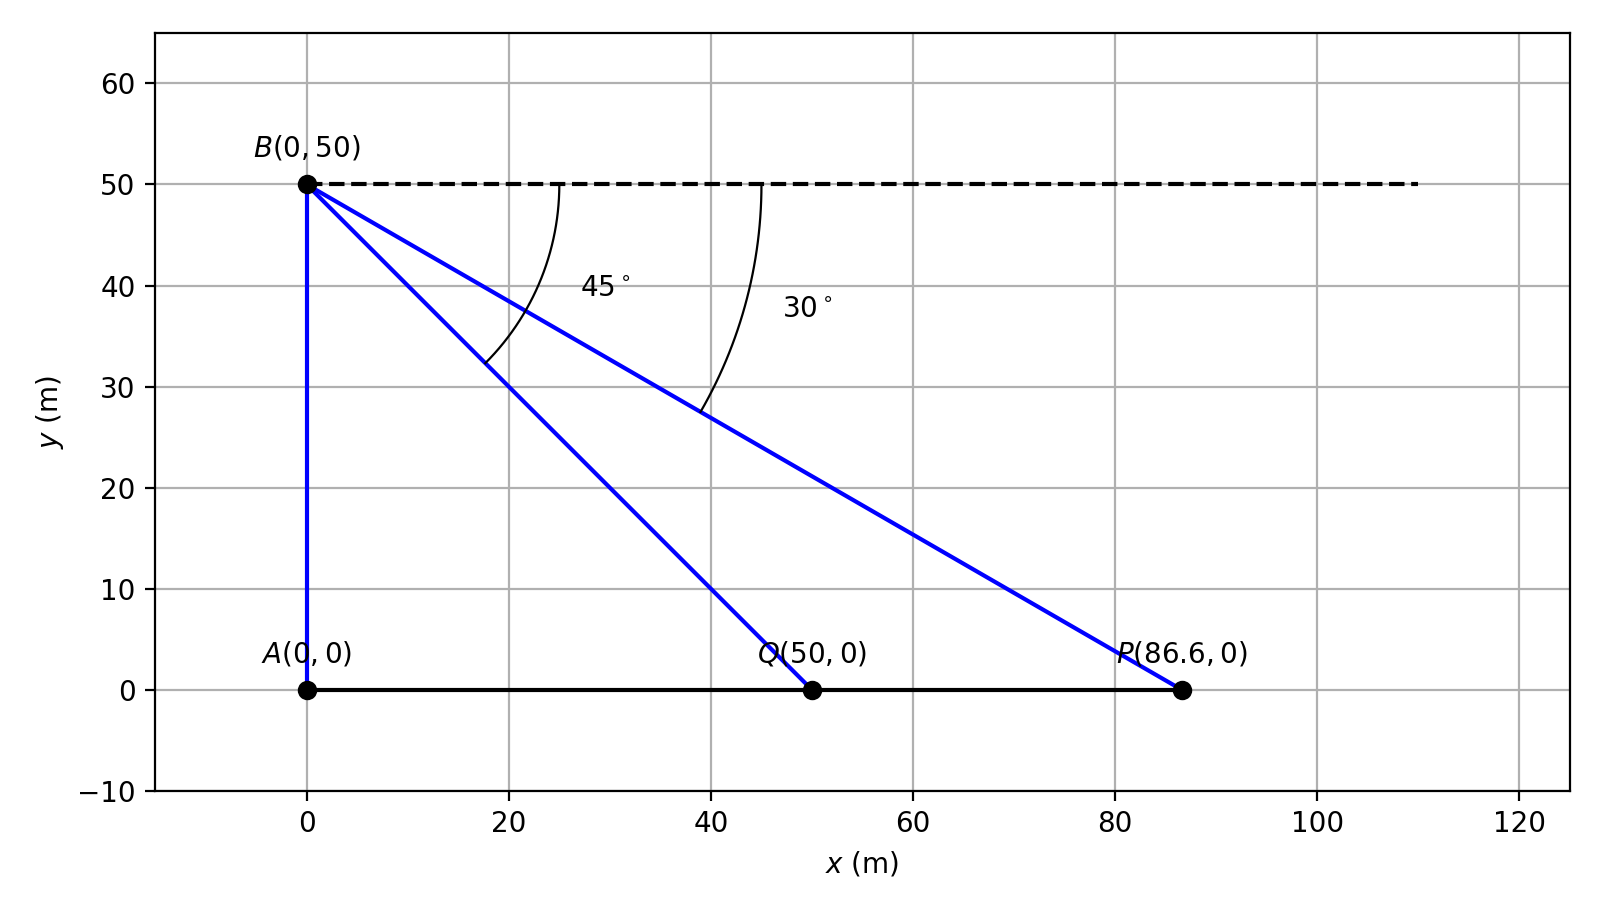
\includegraphics[width=0.8\linewidth]{figs/q38.png}
	\caption{Lighthouse $AB$ and ship positions $P$, $Q$, plotted from coordinates}
	\label{fig:CBSE25S2-q38}
\end{figure}

\end{enumerate}

